\chapter{Estrategia de resolución}

En este capítulo se explica el proceso llevado a cabo para desarrollar la solución. Se presenta el modelado básico del problema que consiste en un mapa de la zona con todos los datos necesarios para realizar la simulación y el algoritmo genético utilizado con su estructura, parámetros y configuración. Se detalla la biblioteca utilizada para el desarrollo del algoritmo genético y la arquitectura propuesta.

La metodología se basa en cuatro puntos que serán tratados a continuación estos son:

\begin{itemize}
	\item Modelado del problema.
	\item Algoritmo genético multiobjetivo y paralelo.
	\item Simulador de tráfico.
	\item Cluster Fing para la ejecución del algoritmo. 
\end{itemize}





\section{Modelado del problema }

Para solucionar el problema se usarán simulaciones de la realidad, por tanto es importante contar con un modelo detallado y fidedigno. A continuación se da información sobre el simulador a utilizar, las herramientas necesarias y el proceso seguido para generar el modelo. 

\subsection{Simulador SUMO (Simulation of Urban MObility)}

Como se explicó en el marco teórico SUMO es un simulador de tráfico gratis y abierto que nos permite modelar redes de calles, vehículos, transporte público, ciudadanos y semáforos \citep{SUMO}. Sigue un modelo microscópico ya que realiza la simulación individual explícita de cada elemento. Incluye un conjunto de herramientas destinadas  a facilitar la generación de tráfico y la construcción de mapas. 

Dado que existe un amplio abanico de posibilidades a la hora de elegir un simulador se realizo un análisis relacionado a las posibilidades y objetivos del proyecto, a continuación se detallan las razones que sustentan la elección de SUMO como el simulador utilizado:

\begin{itemize}
	\item Portable: SUMO puede ser ejecutado tanto en Windows como en Linux, esto es importante dado que son las plataformas en las que se desarrolla el proyecto, ademas el Cluster Fing utiliza el sistema operativo CentOs Linux) y era un requisito que pudiera ser ejecutado en este ambiente.
	
	\item Tipos de ejecución: Permite las opciones de ejecutarse sin interfaz gráfica utilizando la linea de comando lo que aumenta sensiblemente la velocidad de ejecución, ademas esto es fundamental a la hora de realizar la arquitectura necesaria ya que el programa tiene que tener la posibilidad de ejecutar el simulador de manera directa. Por otro lado también tiene la opción de mostrar la interfaz gráfica lo cual es indispensable a la hora de visualizar la simulación sobre todo en los primeros momentos del desarrollo en los cuales se realizan ajustes y pruebas.
	
	\item Gratis y abierto: SUMO es de código abierto y sin costo, el cual es un factor importante para un proyecto de investigación como el que se quiere desarrollar. 
	
	\item Documentación y mantenimiento: Cuenta con una detallada documentación lo cual hace mas fácil su utilización, así como una comunidad muy activa que responden dudas en foros lo que es útil a la hora de buscar soporte si ocurriera algún problema o se detectara un error. También cuenta con un desarrollo activo lo cual es importante pues se realizan correcciones y actualizaciones frecuentemente.
	
	\item Configuración simple: Tiene un sistema sencillo para configurar las simulaciones basada en archivos XML, de esta forma se pueden modificar la configuración de los semáforos, las propiedades de los vehículos, las rutas que estos siguen entre otras opciones. Ademas tiene herramientas para poder utilizar mapas importados de servicios como \citet{OSM}.
	
	\item Información de salida: SUMO tiene la opción de generar una amplia gama de datos producidos por la simulación entre los que se encuentran la velocidad de los vehículos y el largo del recorrido que son requeridas por la solución propuesta. 
	
	\item Eficiente: Soporta redes de transito muy grandes y esta diseñado para ejecutar simulaciones a gran velocidad \citep{sumo2014}. Lo cual es una característica deseable por la complejidad del problema a solucionar.
	
\end{itemize}


Tiene un funcionamiento sencillo basado en tomar como entradas archivos de configuración que representan la red vial, los vehículos, el tráfico y los semáforos. Y archivos de salida con información interesante como el tiempo de simulación, la cantidad de vehículos, sus velocidades, duración del viaje, emisiones de gases contaminantes, etc. 

Algunas otras herramientas relacionadas a la simulación:

\begin{itemize}
	
	\item  NetConvert: Utilizado para la generación de la red a partir de un mapa. Por ejemplo podemos transformar un mapa de Open Street Map en archivo XML de red que SUMO reconoce. Este programa viene integrado con SUMO.
	\item DUaRouter: Genera recorridos de vehículos basado en dinámicas definidas por el usuario. Esta utilidad viene integrada con SUMO.
	\item Traffic Modeler: Herramienta para la generación de tráfico de manera visual y luego exportarlo para que sea reconocido por SUMO. \citep{TrafficModeler}
	
	
\end{itemize}

\begin{figure}[H]
	\centering
	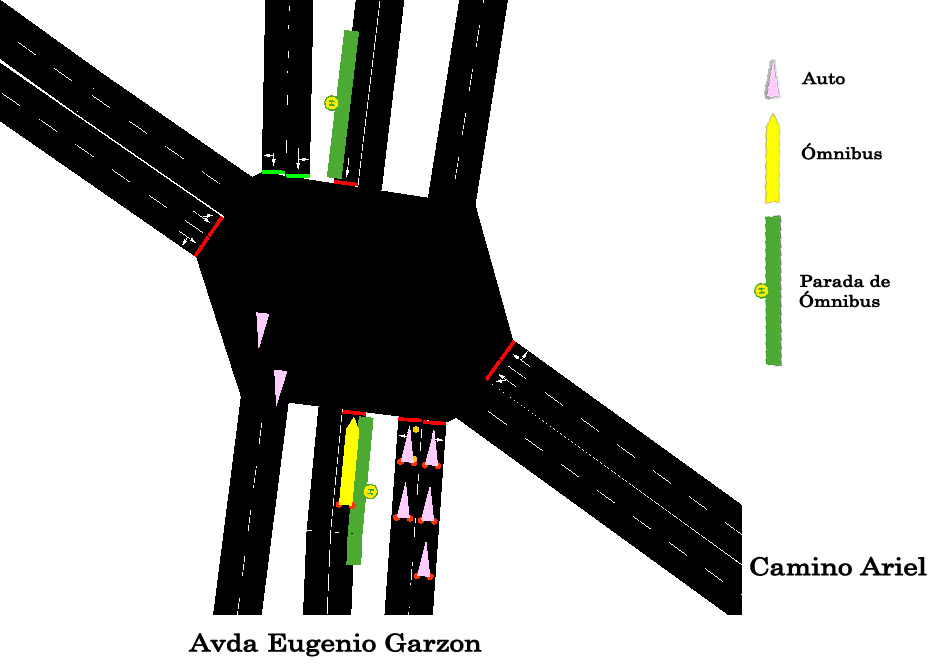
\includegraphics[width=0.7\linewidth]{Figures/sim1}
	\caption{Simulacion de tráfico en SUMO en el cruce entre Bulevar Battle y Ordoñez y el Corredor Garzón.}
	\label{fig:sim1}
\end{figure}



\subsection{Proceso del modelado}

Se describen los pasos realizados para tener los elementos necesarios para realizar la simulación.

\subsubsection{Diseño del mapa}

El primer paso consiste en desarrollar un mapa de la zona que sea compatible con el simulador. Para ello se utiliza el servicio de Open Street Map \citep{OSM} que cuenta con mapas libres y actualizados por una comunidad muy activa. Al notar que calles de una sola mano estaban como doble vías y algunos cruces de Garzón como Lezica, diferían con lo visto in situ, se cotejo la exactitud comparando con otros servicios como Google Maps y Bing Maps que al poseer tambien fotos actualizadas del lugar se podía discernir y recordar de como eran las calles realmente.

Se exporta el mapa al editor \citet{JOSM} para poder adecuarlo a las necesidades del problema. El alcance que se pretende es la zona que corresponde al Corredor Garzón desde su inicio hasta el final y dos caminos paralelas a cada lado. Como se ve en el mapa no existen calles paralelas reales por lo que fue una tarea dificultosa en este aspecto ya que se eligieron primero las calles que corresponderían a las paralelas y todas las calles que permiten ir de una calle a la otra, chequeando que quede una doble mano o dos calles de una mano sola y luego se borraron manualmente todas las demas calles.

\begin{figure}[H]
	\centering
	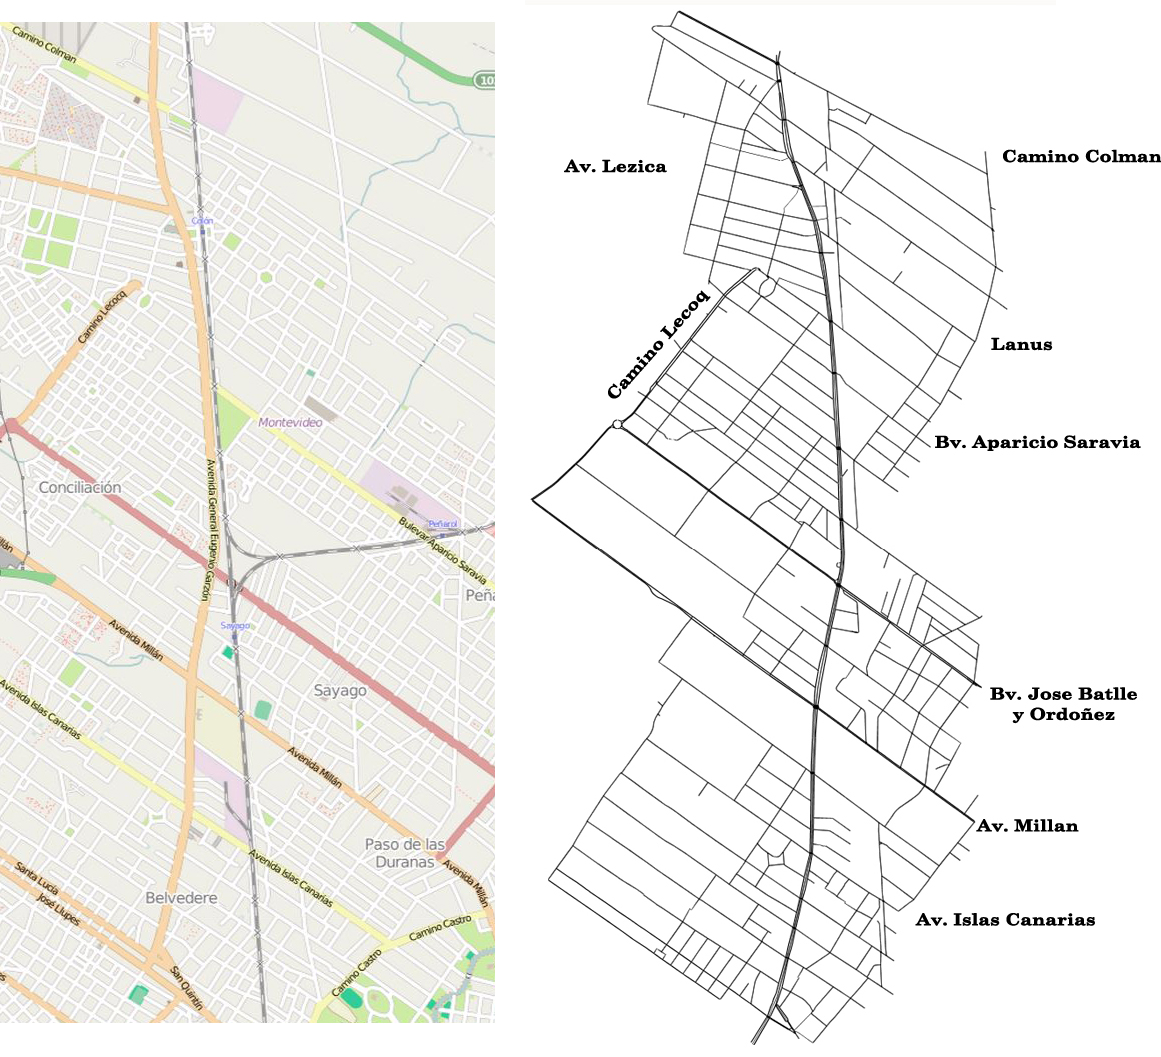
\includegraphics[width=0.7\linewidth]{Figures/mapa_osm_sumo}
	\caption{A la izquierda el mapa extraido de OSM, a la derecha el mapa procesado listo para ser usado en SUMO.}
	\label{fig:mapa_osm_sumo}
\end{figure}

Luego se utilizó la herramienta Netconvert para transformarlo al formato que SUMO acepta, Netconvert no reconoce un monton de datos aportados por el formato OSM como los numeros de casas, las vias del tren, las vías de peatones,los caminos, las paradas, los separadores que tiene el corredor de las vias de autos etc.pero NetConvert no esta hecho para reconocer corredores por lo que mezclaba y superponia el corredor con las vias de los autos, por lo que lo primero que hubo que hacer es separar aproximadamente 1 metro las calles para que NetConvert interpretara que no era posible cambiar entre la via de los autos y del ómnibus (como la realidad)y se realizaron varios ajustes editando los archivos generados para corregir errores en las calles, cruces y conexiones. De esta manera se obtuvo un mapa fiel a la realidad y compatible con el simulador.


\subsubsection{Trabajo de campo}
Se cuentan con los datos públicos sobre la cantidad de  ómnibus y sus frecuencias pero no se tienen datos sobre la densidad de tráfico vehicular en la zona, por esto se realiza un revelamiento in-situ con las siguientes características.

Se seleccionaron cinco cruces que presentan diferentes características para poder modelar variantes en la cantidad de vehículos circulantes.
Estos son: Camino Ariel, Battle y Ordoñez, Plaza Videla, Camino Colman y Aparicio Saravia. 

Se siguen las recomendaciones de los textos consultados al respecto \citep{ConteoTrafico}. Se eligió el día miércoles, que estuviera soleado y entre las 15 y 17 horas para no tener los sesgos que se producen los fines de semana o días de lluvia.
Se realizaron filmaciones de entre 15 y 30 minutos en los cruces y luego se analizaron los vídeos para realizar el conteo manual con la posibilidad de enlentecer el vídeo para mayor facilidad. Luego se completa una planilla electrónica donde se tiene la información de vehículos que recorren Garzón, la calle que cruza y los que doblan. 

\begin{figure}[H]
	\centering
	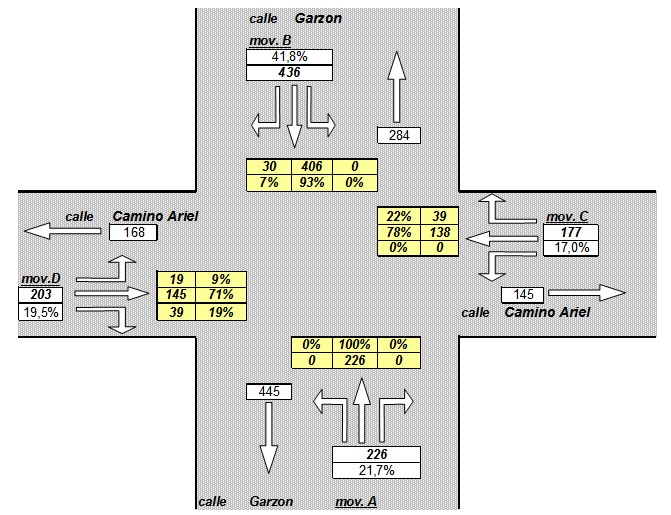
\includegraphics[width=0.7\linewidth]{Figures/conteo_hoja}
	\caption{Ejemplo de planilla electrónica para el conteo manual en Camino Ariel}
	\label{fig:conteo_hoja}
\end{figure}



\begin{table}[h]
	\renewcommand{\arraystretch}{1.2}
	\caption{Resumen del revelamiento del tráfico en la zona del corredor Garzón. Se muestra la cantidad de vehículos  y la orientación hacia donde circulan. }
	\label{table:resumen_trafico}
	\centering
	\begin{tabular}{lcccc}
		\hline
		Intersección&
		Sur-Garzón& 
		Norte-Garzón & 
		Oeste &
		Este 
		\\ 
		\hline
		Camino Colman  & 410 & 390 & 140 & 230\\		
		Plaza Vidiella  & 400 & 444 & 292 & 0\\		
		Aparicio Saravia  & 390 & 450 & 40 & 90\\		
		Battle y Ordoñez  & 510 & 390 & 470 & 300 \\	
		Camino Ariel  & 436 & 226 & 177 & 203 \\													
		\hline
		
		
		\hline
	\end{tabular}
\end{table}


Además se realizaron recorridas de punta a punta del corredor a una velocidad constante en auto para verificar los tiempos obtenidos en la simulación.

Para obtener la configuración de los semáforos se realizó un recorrido en bicicleta por el corredor cronometrando la duración del tiempo en cada esquina de cada semáforo. Tanto de ida como de vuelta para corroborar que fueran correctos. Estos tiempos fueron verificados por los vídeos obtenidos.


\newpage
\subsubsection{Modelo del tráfico}
Una vez que se tiene el mapa compatible con el simulador y los datos relevados de la realidad se agrega el tráfico a la simulación.

Existen varios modelos disponibles para la representación de la circulación de vehículos, aquí exponemos algunos de los más populares. 
\begin{itemize}
	\item Aleatorios: Genera diferentes recorridos que seguirán los vehículos aleatoriamente
	\item Basado en áreas:  Se especifican áreas como un conjunto de calles y se realizan recorridos entre ellas.
	\item Basado en Actividad: Se especifica la cantidad de casas, vehículos y población en un determinado lugar y el modelo genera la densidad de tráfico que se producirá basado en los tipos de actividades que se realizan comúnmente como ir al trabajo, hacer las compras, ir a la escuela,  etc
	\item Definido por el usuario: que permiten determinar la ruta de los vehículos con mayor detalle.
\end{itemize}


Se utilizó el programa Traffic Modeler \citep{TrafficModeler} que sirve para generar modelos de tráfico complejos de manera visual. Se optó por un modelo de movilidad entre áreas lo que permite una buena granularidad al especificar la densidad de tráfico.


\begin{figure}[h]
	\centering
	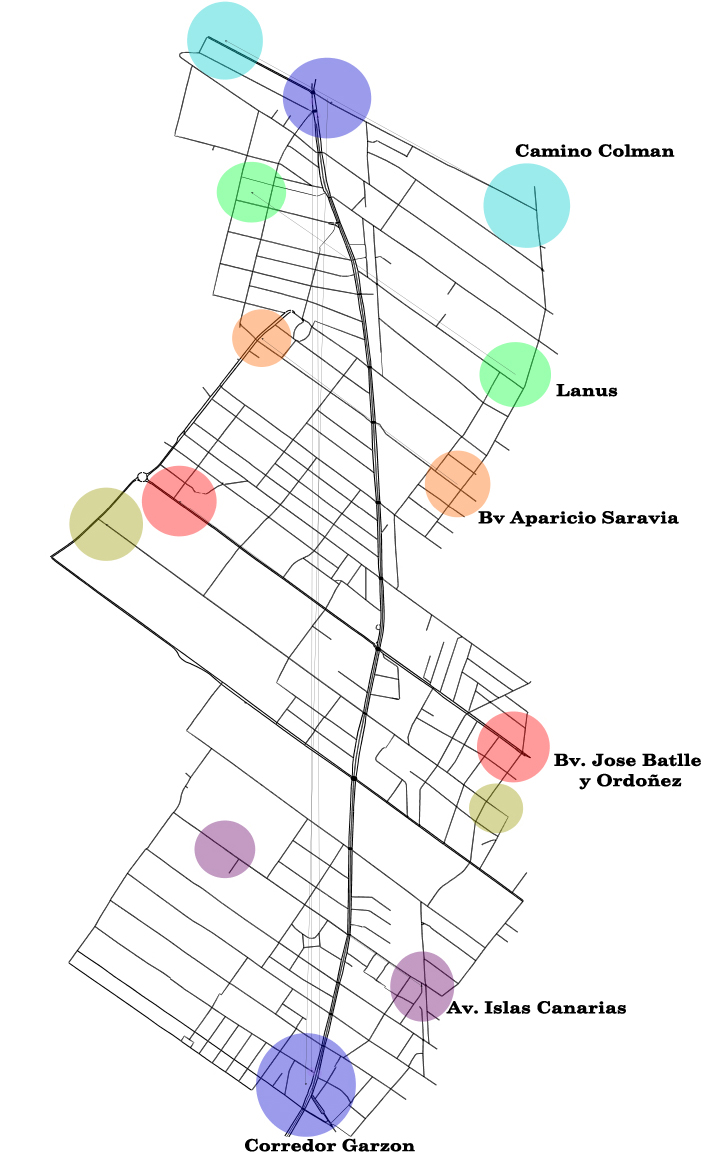
\includegraphics[width=0.3\linewidth]{Figures/areaflow1}
	\caption{Mapa del TrafficModeler con las áreas de tráfico. Círculos del mismo color indican tráfico especificado entre esas áreas}
	\label{fig:areaflow1}
\end{figure}


Se manejaron dos tipos de vehículos autos y ómnibus cada uno con características distintas tanto de tamaño, aceleración y velocidad máxima.

Se agregaron las frecuencias y los distintos recorridos de los ómnibus obtenidos de datos públicos de la Intendencia Municpal de Montevideo \citep{IMM}
Estos incluyen las líneas urbanas  'G', '409' ,'2', 'd5'  y  '148'. 

Las líneas de ómnibus suburbanas realizan  un mismo  trayecto y las generalizamos con el nombre 'A' las cuales no van a ser tomadas en cuenta en la optimización del algoritmo pero si aparecerán en la simulación.

La ubicación y líneas de cada parada se obtuvo de \citep{sigMontevideo}, existen 14 paradas para líneas urbanas por el corredor para el recorrido de ida y las mismas para la vuelta.
Para los recorridos se hicieron  variantes  en  los  viajes  dentro  de  una  misma línea para simular el hecho de que no siempre se para en las mismas paradas.

También se tuvo en cuenta para la simulación el tiempo que demora un ómnibus al detenerse en una parada, y que hay algunas donde por la cantidad de gente se demora más. Estos datos fueron obtenidos en el lugar considerando tiempos de entre 15 a 35 segundos.

Para establecer la velocidad media de los ómnibus se realizó un estudio basado en datos de GPS proporcionados por la IMM luego de reuniones con Ingeniería de Tránsito.
Estos datos cuentan con la posición GPS, la velocidad instantánea y la referencia al ómnibus para un conjunto de líneas seleccionadas tomadas en un período de una semana. Luego de procesar los datos se obtuvo una velocidad media de 14.5 km/h lo que permite ajustar mejor el modelo. 

Para introducir estos datos en el simulador se utilizan tres archivos de configuración en formato xml que son tomados como entrada, estos son:

\begin{itemize}
	\item Semáforos: Cuenta con la información detallada de la duración de los semáforos, el comienzo de su fase y la ubicación del mismo respecto al mapa base.
	\item Rutas de vehículos: Se indica la ruta de cada vehículo que recorrerá el mapa.
	\item Recorrido de ómnibus: Indica las rutas de los ómnibus, la frecuencia, la ubicación de las paradas, en cuales se detiene y cuanto demora.
\end{itemize}




\section{Arquitectura de la solución}

En la figura \ref{fig:arquitectura1} se muestra la arquitectura propuesta para el problema.

La biblioteca Malva se utiliza para la implementación del algoritmo, en cada evaluación de la función de fitness se realiza un llamado al simulador SUMO. 

En el primer paso el algoritmo genera la población inicial, estos individuos representan una configuración de semáforos para el Corredor con el tiempo de duración de las luces y las fases. Esta población se genera realizando algunas variaciones de los valores reales obtenidos.

\begin{figure}[H]
	\centering
	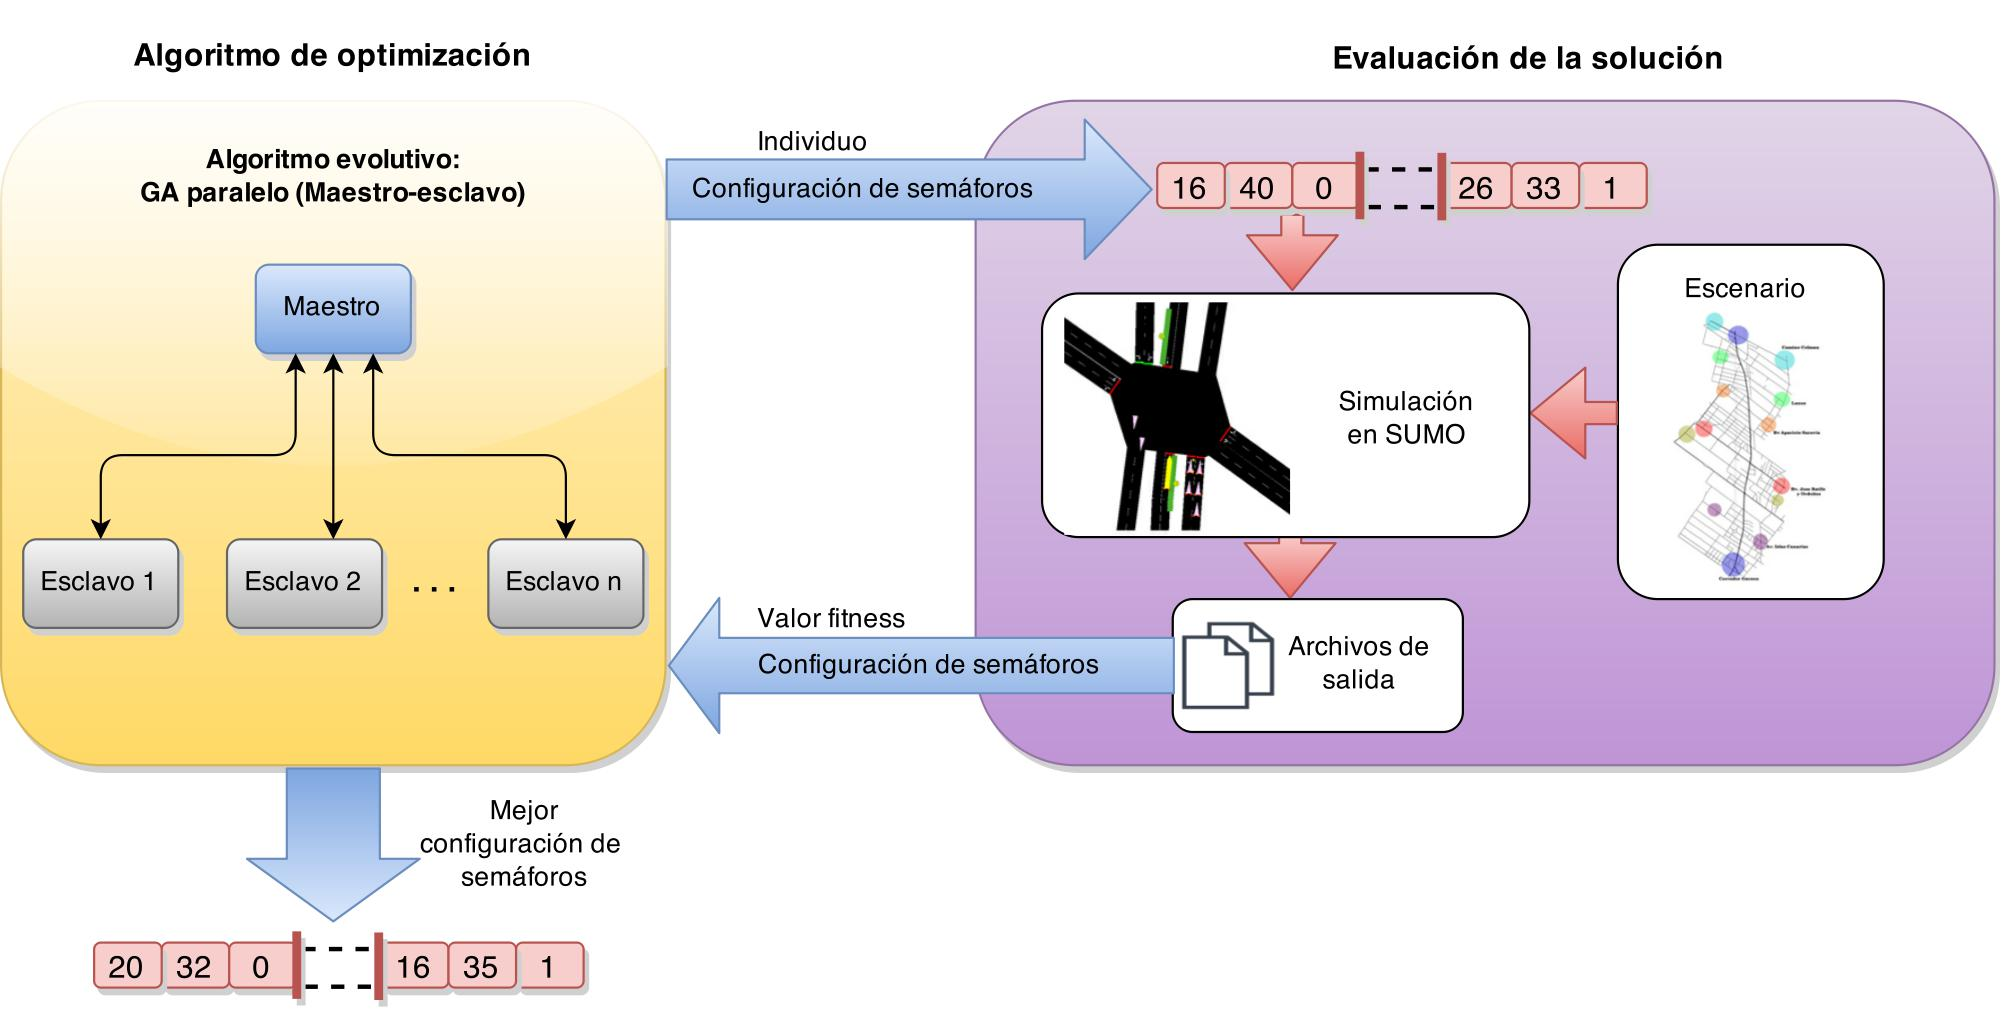
\includegraphics[width=0.7\linewidth]{Figures/arquitectura1}
	\caption{Arquitectura de la función de fitness}
	\label{fig:arquitectura1}
\end{figure}

Luego por cada individuo se genera un archivo compatible con el simulador que representa la configuración de semáforos. Este archivo se utiliza como entrada para ejecutar el simulador para cada individuo. Al finalizar la ejecución se generan archivos de salida que son procesados por el algoritmo, estos tienen la información necesaria para calcular el fitness de cada individuo como la velocidad media de ómnibus y otros vehículos.


\section{Implementación: Biblioteca Malva}

Dada la complejidad del problema se tuvo en cuenta desde un primer momento la utilización de un \emph{framework}, de esta forma se podría lograr una ejecución eficiente y una implementación robusta pero flexible. 

Como se detalló en el marco teórico existen varias opciones de \emph{frameworks} disponibles. Por las particularidades del problema existen ciertos requerimientos a la hora de seleccionar  uno para su resolución, entre los que se destacan:

\begin{itemize}
	\item Abierto y gratuito: Al ser un proyecto de investigación de índole académico es conveniente que no se tengan costos económicos asociados. Ademas es importante que se cuente con el código abierto con el fin de introducir modificaciones en el código base o corregir errores.
	\item Algoritmo genético: El framework debe facilitar el desarrollo de un algoritmo genético ya que es la base en la que se sustenta el proyecto.
	\item Algoritmo paralelo: Por la complejidad del problema y el alto consumo de recursos computacionales que insume es fundamental la opción de ejecución en paralelo. Sino cuenta con funcionalidad nativa al menos que tenga la posibilidad de modificar el código principal para agregarlo.
	\item Plataforma: Es requerido que se pueda ejecutar en el Cluster Fing (CentOs - Linux), en Windows y otros sistemas Linux, ya que son las plataformas en donde se desarrollará el trabajo.
	\item Confiabilidad: Es deseable que sea lo suficientemente estable como para tener confianza de que el algoritmo funcionara sin demasiados problemas de manera correcta. Por ejemplo que existan casos de éxito usando el \emph{framework}, documentación , ejemplos de código, etc.
	\item Lenguaje: Es deseable que esté desarrollado en c++ o java por la experiencia que se cuenta en estos lenguajes. 
	\item Multiobjetivo: Es deseable aunque no requerido que soporte algoritmos multiobjetivo, ya que la función que se quiere implementar aun siendo multiobjetivo es sencilla.	
\end{itemize} 

Luego de analizar todos estos puntos se selecciona la biblioteca Malva para la implementación del algoritmo. A continuación se detalla su funcionamiento y características.


Como se explico anteriormente \citet{Malva} surge como una variante del proyecto \citet{Mallba}.Propone su actualización, mejora y desarrollo como un proyecto de código abierto colaborativo.  Su objetivo es proveer de varios esqueletos de  heurísticas de optimización que puedan ser utilizados y extendidos de manera fácil y eficiente.

Los esqueletos se basan en separar dos conceptos: El problema concreto que se quiere resolver y por otro lado el método utilizado para resolverlo. Por tanto un esqueleto se puede ver como una plantilla genérica que se instancia para resolver un problema particular, manteniendo todas las funcionalidades genéricas.

Utiliza el lenguaje c++ dado su alto nivel, modularidad y flexibilidad. Los esqueletos se ofrecen como un conjunto de clases requeridas que son las que el usuario deberá modificar para adaptarlo a su problema y las provistas que incluyen todos los aspectos internos del esqueleto y son independientes del problema particular. Entre los algoritmos provistos se encuentra el de Algoritmos genéticos y \citet{CHC}.



\newpage

\section{Especificación del Algoritmo Genético utilizado}
Se utiliza el algoritmo genético provisto por la biblioteca  Malva  llamado NewGA al cual se le realizan algunas modificaciones para lograr su ejecución en paralelo, con el objetivo de reducir los tiempos de ejecución del algoritmo ya que los escenarios planteados se consideran complejos y que insumirán una gran carga de recursos computacionales.

Se utiliza el método maestro-esclavo donde el maestro se encarga de la mayoría de las funciones:

\begin{itemize}
\item Inicialización de la población.
\item Distribuir la evaluación de los individuos hacia los esclavos creando un hilo por cada esclavo	.
\item Obtener de los esclavos los valores obtenidos de fitness.
\item Selección de los mejores individuos.
\item Aplicación de operadores de cruzamiento y mutación.
\item Reemplazo y generación de la siguiente población.
\end{itemize}

Mientras los esclavos se encargan solamente de lo siguiente:
\begin{itemize}
	\item Obtener el individuo enviado por el maestro.
	\item Ejecutar la evaluación del individuo que corresponde a ejecutar el simulador y obtener los datos de salida.
\end{itemize}


El siguiente esquema muestra el algoritmo utilizado. 

\begin{algorithm}[H]
	\caption{Algoritmo Genético de Malva. }
	\label{alg:algoritmo_genetico_malva}
	\begin{algorithmic} [1] 
		{
			\STATE \texttt{t} = 0
			\STATE {Inicializo( P(t))}
			\STATE {Evaluar estructuras en ( P(t))}			
			\WHILE {\text{No termine}}
			\STATE \texttt{t}++		
			\STATE {Seleccionar C(t) de P(t-1)}	
			\STATE {Recombinar estructuras en C(t) formando C'(t)}				
			\STATE {Mutar estructuras en C'(t) formando C''(t)}		
			\STATE {Evaluar estructuras en C''(t) generando un hilo de ejecucion por cada una}					
			\STATE {Consolidar valores de la evaluacion}								
			\STATE {Reemplazar P(t) de C''(t) y P(t-1)}								
			\ENDWHILE
		}
	\end{algorithmic}
	
\end{algorithm}

A continuación se realiza un resumen de las características del algoritmo implementado, que en la siguiente sección serán tratados en mayor detalle:
\begin{itemize}

\item Algoritmo paralelo: Utiliza el método maestro-esclavo para que en cada iteración el maestro genere un hilo para cada ejecución  de la función fitness y luego espere a la terminación de todos los hilos para consolidar los datos. 
\item Función Multiobjetivo: Se intenta optimizar tanto la velocidad promedio de vehículos como de ómnibus teniendo cada uno un peso especifico.
\item Representación del cromosoma: Es un vector de números reales que representan los tiempos de los semáforos y sus fases.
\item Cruzamiento y mutación: Se utiliza una variante del cruzamiento de un punto especifico para el problema al igual que para la mutación.
\item Selección y reemplazo: Reemplaza padres por hijos, la selección de los padres se realiza por el método de torneo de tres individuos y la selección de hijos por el método de ruleta.

\end{itemize}






 

\subsection{Representación del cromosoma}

Definimos los siguientes conceptos:
\begin{itemize}
	\item Cruce: Es el lugar de intersección de dos o más vías de circulación.
	\item Fase: Es la configuración de las luces de los semáforos en un determinado cruce.
\end{itemize}


El  cromosoma  se  va  a  agrupar  lógicamente  en  cruces siendo el valor de cada gen el tiempo que demora una
fase de un cruce, además se agrega para cada cruce un número que representa en que fase comenzará el semáforo. 
Por tanto el tamaño del cromosoma depende tanto de la cantidad de cruces como de la cantidad de fases de cada uno.

En la representación se omiten las luces amarillas ya que no modifican los tiempos reales del paso de vehículos.
 
 \begin{figure}[h]
 	\centering
 	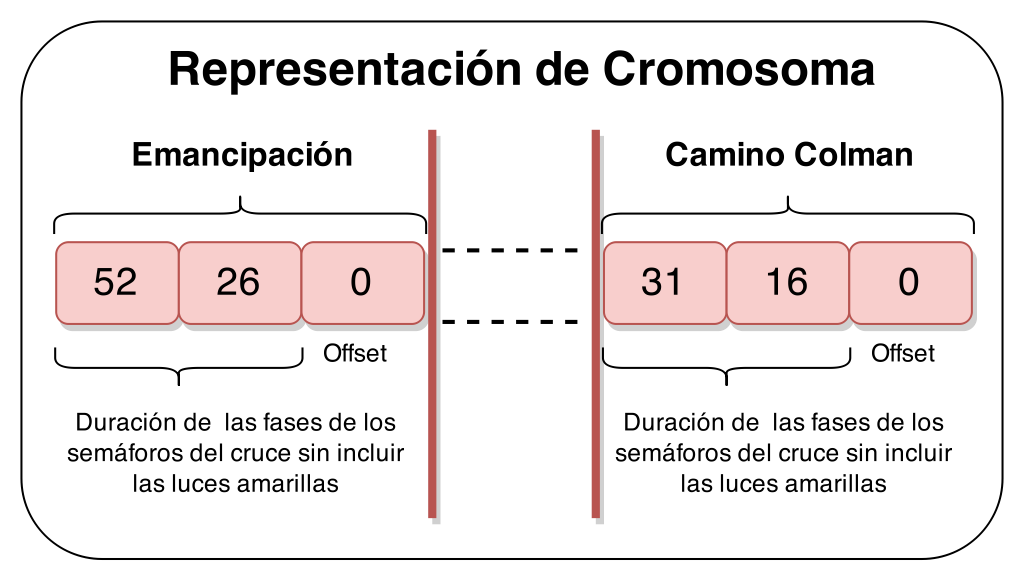
\includegraphics[width=0.7\linewidth]{Figures/cromosoma1}
 	\caption{Cromosoma de 2 cruces}
 	\label{fig:cromosoma1}
 \end{figure}
 
Es  importante que el algoritmo no genere soluciones inviables por lo que no debe modificar la combinación de luces de cada fase para evitar combinaciones de luces erróneas. Por tanto la modificación se realizará solo en el valor que indica el comienzo de fase y en los tiempos relacionados.

\begin{figure}[H]
	\centering
	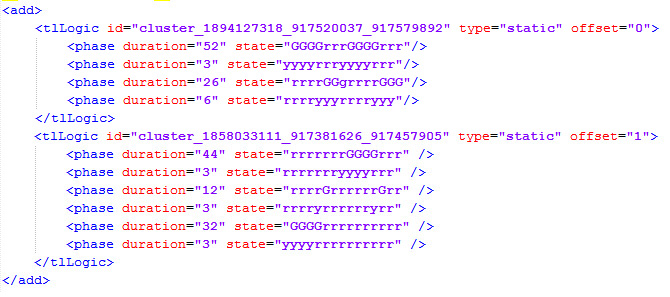
\includegraphics[width=\linewidth]{Figures/rep_sumo2}
	\caption{Representación de Sumo}
	\label{fig:rep_sumo}
\end{figure}

En la figura \ref{fig:rep_sumo} vemos el archivo con la configuración de semáforos que utiliza el simulador para el cromosoma anterior, donde se representan las fases. Por ejemplo el estado \emph{GGGGrrrGGGGrrr} indica la secuencia de luces y su duración de 52 segundos. \emph{G} indica la luz verde, \emph{r} la roja, \emph{y} el Amarillo. El offset indica el inicio de la fase. 

En la figura \ref{fig:sem_numerados} se numeran los semáforos que se corresponden con la primera fase de este ejemplo, donde cada posición de la secuencia \emph{estado} se corresponde a un color en particular. 
\newpage

Por tanto para \emph{GGGGrrrGGGGrrr} tenemos que:
\begin{itemize}
\item GGGG se corresponde a 1, 2, 3 y 4. 
\item rrr a 5, 6 y 7. 
\item GGGG a 8, 9, 10 y 11. 
\item rrr a 12, 13 y 14. 
\end{itemize}
  




\begin{figure}[H]
	\centering
	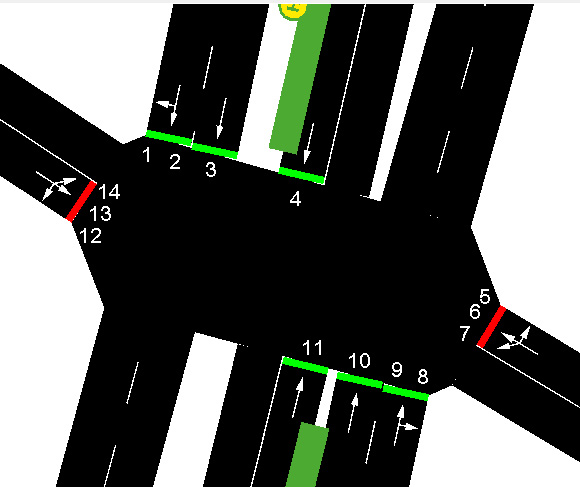
\includegraphics[width=0.7\linewidth]{Figures/semaforos_numerado}
	\caption{Representación de una fase de los semáforos para un cruce. Cada número se corresponde a una letra en la secuencia de \emph{state} del archivo de configuración del simulador SUMO.}
	\label{fig:sem_numerados}
\end{figure}

\subsection{Población inicial}

Para la inicialización de la población se toma como referencia
la configuración obtenida con los datos in-situ, luego para cada
cruce se hacen variar las duraciones de las fases de manera aleatoria entre un rango de valores configurable. Se elige la fase inicial aleatoriamente entre la cantidad de fases del cruce.

\subsection{Función fitness}
La evaluación de un individuo se realiza generando un archivo con la configuración de los semáforos en base a su cromosoma y ejecutando el simulador SUMO utilizando esta configuración para luego obtener los tiempos necesarios para calcular el fitness.

Se empleará una función multiobjetivo usando combinación lineal de la velocidad de los ómnibus y del resto de los vehículos, ya que es un método sencillo y adecuado cuando son menos de tres objetivos. El fitness se calcula como una suma ponderada, con los pesos fijados a priori.

        \begin{equation}
        \label{eq:funcion_fitness_generica}
		F(x) = \sum_{i=1}^{n}{w_i}{f_i}(x)
        \end{equation}

En nuestro caso tenemos como objetivo la velocidad promedio de los ómnibus (vpb) y la velocidad promedio del resto de los vehículos (vpv).

Esta es la formula de fitness donde \emph{x} e \emph{y} indica el peso que le vamos a especificar a la función. 

        \begin{equation}
        \label{eq:funcion_fitness}
        f = x.vpb + y.vpv
        \end{equation}
        
En una primera instancia se establece x = y = 1 más adelante se experimentará con otros pesos.

\subsection{Operadores}
\subsubsection{Operador de Cruzamiento}
Se  utilizará cruzamiento de un punto, seleccionando del cromosoma una posición aleatoria entre dos cruces como punto de corte, por tanto si un tramo del corredor tiene un buen comportamiento se intentará mantener esta propiedad.

En la siguiente figura los padres cuentan con tres cruces, se elige un punto de corte aleatoriamente entre dos cruces y se generan los hijos que son una combinación de los padres.

\begin{figure}[H]
	\centering
	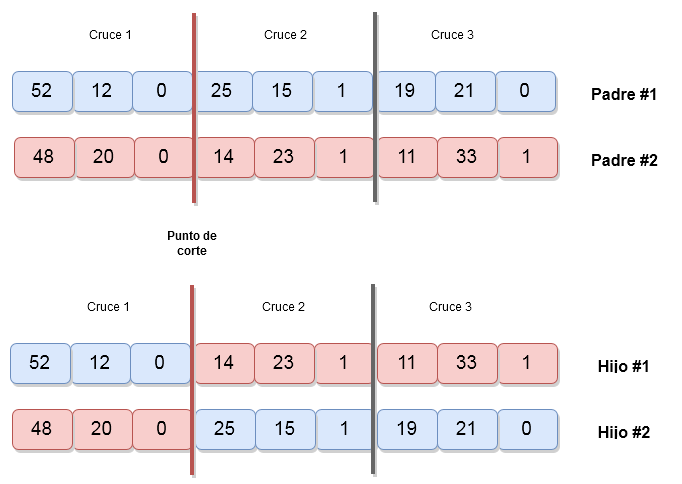
\includegraphics[width=8cm]{Figures/alg_cruzamiento}
	\caption{Visualización del cruzamiento entre individuos.}
	\label{fig:op_cruzamiento}
\end{figure}


\newpage
\subsubsection{Operador de Mutación}
Se implementaron dos tipos de mutación:
\begin{itemize}

\item Mutación de duración de fase: para cada fase de cada cruce se
hace variar su duración sumando o restando una cantidad dada
de segundos entre un rango determinado con una probabilidad
dada.
\item Mutación de inicio de fase: se elige aleatoriamente una fase
con la cual va a comenzar inicialmente el cruce con una probabilidad dada.

\end{itemize}

\subsubsection{Operador de selección y reemplazo}
Se  utilizan los provistos por el algoritmo newGA de Malva. La selección de padres se realiza por el método de torneo de tres individuos y la selección de hijos por el método de ruleta. La política de reemplazo indica que tanto padres como hijos pueden ser parte de la siguiente generación, por lo que existe reemplazo de padres por hijos.

\subsubsection{Parámetros del algoritmo}
Los parámetros específicos del algoritmo se establecen en la siguiente sección, donde se realiza un análisis experimental para encontrar los más adecuados. Estos parámetros son: número de generaciones, tamaño de población, probabilidad de cruzamiento y de mutación.